Using \grp{} (\GRP) as a benchmark, a different communication strategy was tested in this section: the communication of the current configuration in order to avoid its neighborhood, \ie a {\it tabu} configuration.

\subsection{Problem definition}

The \grp{} (\GRP) problem consists in finding an ordered vector of $n$ distinct non-negative integers, called \textit{marks}, $m_1 < \dots < m_n$, such that all differences $m_i - m_j$ $(i > j)$ \new{called \textit{measures}} are all different. An instance of this problem is the pair $(o,l)$ where $o$ is the order of the problem, (\ie the number of \textit{marks}) and $l$ is the length of the ruler (\ie the last {\it mark}). We assume that the first \textit{mark} is always 0. This problem has been applied to radio astronomy, x-ray crystallography, circuit layout and geographical mapping \cite{Soliday1995}. 
When \posl{} is applied to solve an instance of this problem sequentially, it can be noticed that it performs many {\it restarts} before finding a solution, as Table~\ref{tab:golomb_sec_notabu} shows. For that reason this problem was chosen to study a new \commstr.

The cost function is implemented based on the storage of a counter for each measure present in the rule (configuration). All measure where a variable is participating are also stored. This information is useful to compute the more culprit variable (the variable that interferes less in the represented measures), in case of the user wants to apply algorithms like Adaptive Search. 
\new{To compute the cost of a configuration, a differences triangle is built similar to the one introduced in previews section stuying \carrp. This differeces triangle represents all possible measures present in the rule. Se the following example:}

\poslexample{Figure~\ref{fig:ex_golomb} shows all possible measures that the rule represented through the configuration $s=\{0, 1, 4, 9, 11\}$ of order $o$ can measure. So, its corresponding differences triangle is the following:
\begin{equation*}
\begin{tabular}{cll}
0\hspace{10pt}1\hspace{10pt}4\hspace{10pt}9\hspace{7pt}11 & $\rightarrow$ & $s$\\
1\hspace{10pt}3\hspace{10pt}5\hspace{10pt}2 & $\rightarrow$ & $d_1$ \\
4\hspace{10pt}8\hspace{10pt}7 & $\rightarrow$ & $d_2$ \\
9\hspace{7pt}10 & $\rightarrow$ & $d_3$ \\
11 & $\rightarrow$ & $d_4$
\end{tabular}
\end{equation*}
where each measure in $d_k$ are the vector of measures $s_{i+k} - s_i$, for all $k \in [0, o-i-1]$.
}

\begin{figure}[h]
\centering
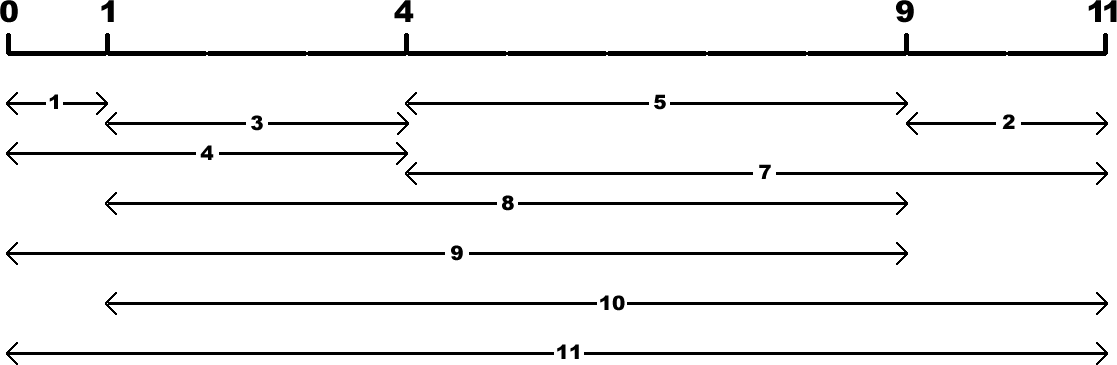
\includegraphics[width=0.7\linewidth]{golomb.png}
\caption[]{Golomb ruler of order 5 and length 11}
\label{fig:ex_golomb}
\end{figure}

\new{The cost is calculated as the number of equal measures present in the differences triangle. It is easy to prove that checking this triangle until the row $d_B$, with $B=\floor*{(o-1)/2}$ is enough. So, the cost can be calculated in $O\left(o^2\right)$.} %$O\left(o^2 + l\right)$.

\subsection{Experiments design and results}

\grp{} instances were used to study a different \commstr. This time the current configuration is communicated to avoid its neighborhood, \ie a {\it tabu} configuration. Some modules used in the resolution of \sg{} and \carr{} problems have been reused to design the solvers: the \textit{Selection} and \textit{Acceptance} modules. The new modules are:

\begin{enumerate}
	\item$I_{sort}$: returns a random configuration $s$ as an increasing ordered vector of integers. The configuration is generated \textit{far} from the set of {\it tabu} configurations arrived via solver-communication, in communicating strategies (based on the \textit{generation} \absm{} $I$).
	\item $V_{sort}$: given a configuration, returns the neighborhood $V\left(s\right)$ by changing one value while keeping the order, \ie replacing the value $s_i$ by all possible values $s'_i \in D_i$ satisfying $s_{i-1} < s'_i < s_{i+1}$ (based on the \textit{neighborhood} \absm{} $V$).
\end{enumerate}

An abstract module $R$ for reset was also added: it receives and returns a configuration. The concrete reset module used for this problem ($R_{tabu}$) inserts the input configuration into a \textit{tabu} list inside the solver and returns the input configuration as-is. \new{This way it cam be assambled inside the cyclical operator, as Algorithm~\ref{as:golomb_tabu} shows}. This module is executed just before performing a restart, so if the solver was unable to find a better configuration around the current one, this current configuration is assumed to be a local minimum, and it is inserted into a tabu list. \new{Then, in the next iteration, the solver generates a first configuration far enough from all tabu configurations inside the tabu list.} Algorithm~\ref{as:golomb_notabu} and~\ref{as:golomb_tabu} present both solvers, respectively without and with a tabu list. They were used to obtain results presented in Tables~\ref{tab:golomb_sec_notabu} and~\ref{tab:golomb_sec_tabu} to show that the approach explained above provides some gain in terms of runtime \new{but also in terms of percentage of success. As we can see, the runtime improvement is not substantial. The reason is because the solver using a tabu list, can insert one configuration only in the tabu list after each restart.} 

\begin{algorithm}[H]
\dontprintsemicolon
\SetNoline
\SetKwProg{myproc}{\tet{\bf abstract solver}}{\tet{\bf begin}}{\tet{\bf end}}
\myproc{as\_golomb\_notabu \tcp*{{\sc Itr} $\rightarrow$ number of iterations}
	\tet{\bf computation} : $I, V, S, A$\;}{
	\whileinline{$\left(\textbf{\Iter < } K_1\right)$}{
		$I \poslop{\mapsto}$ 
		\whileinline{$\left(\textbf{\Iter \% } K_2\right)$}{$\left[V \poslop{\mapsto} S \poslop{\mapsto} A\right]$}
	}
}
\tet{\bf solver} \solverposl{notabu} \tet{\bf implements} as\_notabu\;
\algoindent \tet{\bf computation} : $I_{sort}, V_{sort}, S_{first}, A_{AI}$ \;
%\tet{\bf connection}: $CM_{last}$\;
\caption{Solver without using tabu list, for \GRP}\label{as:golomb_notabu}
\end{algorithm}

\begin{algorithm}[H]
\dontprintsemicolon
\SetNoline
\SetKwProg{myproc}{\tet{\bf abstract solver}}{\tet{\bf begin}}{\tet{\bf end}}
\myproc{as\_golomb\_tabu \tcp*{{\sc Itr} $\rightarrow$ number of iterations}
	\tet{\bf computation} : $I, V, S, A, R$\;}{
	\whileinline{$\left(\textbf{\Iter < } K_1\right)$}{
		$I \poslop{\mapsto}$ 
		\whileinline{$\left(\textbf{\Iter \% } K_2\right)$}{$\left[V \poslop{\mapsto} S \poslop{\mapsto} A\right]$} $\poslop{\mapsto} R$
	}
}
\tet{\bf solver} \solverposl{tabu} \tet{\bf implements} as\_tabu\;
\algoindent \tet{\bf computation} : $I_{sort}, V_{sort}, S_{first}, A_{AI}, R_{tabu}$ \;
%\tet{\bf connection}: $CM_{last}$\;
\caption{Solver using tabu list, for \GRP}\label{as:golomb_tabu}
\end{algorithm}

\begin{table}[h]
	%\captionsetup{belowskip=6pt,aboveskip=6pt}
	\centering 
	\renewcommand{\arraystretch}{1}
		\begin{tabular}{p{2cm}|R{1.2cm}R{1.2cm}|R{1.5cm}R{1.5cm}|R{0.8cm}R{1.2cm}|R{2cm}}
			\hline 	
			{\bf Instance} & T & T(sd) & It. & It.(sd) & R & R(sd) & \% success\\
			\hline
			8--34 & 0.79 & 0.66 & 13,306 & 11,154 & 66 & 55.74 & 100.00\\
			10--55 & 66.44 & 49.56 & 451,419 & 336,858 & 301 & 224.56 & 80.00\\		
			11--72 & 160.34 & 96.11 & 431,623 & 272,910 & 143 & 90.91 & 26.67\\
			\hline
		\end{tabular}
	\caption{A single sequential solver without using tabu list for \GRP}
	\label{tab:golomb_sec_notabu}
\end{table}

\begin{table}[h]
	%\captionsetup{belowskip=6pt,aboveskip=6pt}
	\centering 
	\renewcommand{\arraystretch}{1}
		\begin{tabular}{p{2cm}|R{1.2cm}R{1.2cm}|R{1.5cm}R{1.5cm}|R{0.8cm}R{1.2cm}|R{2cm}}
			\hline 	
			{\bf Instance} & T & T(sd) & It. & It.(sd) & R & R(sd) & \% success\\
			\hline
			8--34 & 0.66 & 0.63 & 10,745 & 10,259 & 53 & 51.35 & 100.00 \\			
			10--55 & 67.89 & 50.02 & 446,913 & 328,912 & 297 & 219.30 & 88.00\\
			11--72 & 117.49 & 85.62 & 382,617 & 275,747 & 127 & 91.85 & 30.00\\
			\hline
		\end{tabular}
	\caption{A single sequential solver using tabu list for \GRP}
	\label{tab:golomb_sec_tabu}
\end{table}








%When we use \oneTone{} communication, after the restart $k$, the receiving solver has twice the number of configurations in the tabu list (one tabu configuration from itself and the received one after each restart).

\begin{table}[h]
%\captionsetup{belowskip=6pt,aboveskip=6pt}
\centering 
\renewcommand{\arraystretch}{1}
\begin{tabular}{p{2cm}|R{1.2cm}R{1.2cm}|R{1.5cm}R{1.5cm}|R{0.8cm}R{1.2cm}}
	\hline 	
	{\bf Instance} & T & T(sd) & It. & It.(sd) & R & R(sd)\\
	\hline
	%\hline
	8--34 & 0.43 & 0.37 & 349 & 334 & 1 & 1.64\\
	10--55 & 4.92 & 4.68 & 20,504 & 19,742 & 13 & 13.07\\
	11--72 & 85.02 & 67.22 & 155,251 & 121,928 & 51 & 40.64\\
	\hline
\end{tabular}
\caption{Parallel solvers using tabu list for \GRP}
\label{tab:golomb_par_tabu}
\end{table}

\separation

\new{Results in Table~\ref{tab:golomb_par_tabu} show once again the success of the parallel approach. Although this time the improvement with respect to the sequential approach was significant, and tacking into account that \posl{} needs to perform some restarts for solving this problem, a different \commstr{} is proposed. Up to now, in all previews \commstrs{} the current configuration was communicated in order to have more solvers searching in its neighborhood, as an intensification mechanism. In the following \commstr{} the current configuration is communicated when it can be considered as a local minimum. Then, receivers solvers avoid it, by generating starting configurations far enough from it}. The current configuration is considered as a local minimum since the solver (after a given number of iteration) is not able to find a better configuration in its neighborhood, so it communicates this configuration just before performing the restart. 

Algorithm~\ref{as:golomb_sender} presents the sender solver and Algorithm~\ref{as:golomb_receiver} presents the receiver solver. Based on the connection operator used in the communication strategy, this solver might receives one or many configurations. These configurations are the input of the generation module ($I$), and this module inserts all received configurations into a {\it tabu} list, and then generates a new first configuration, far from all configurations in the {\it tabu} list.

\begin{algorithm}
\dontprintsemicolon
\SetNoline
\SetKwProg{myproc}{\tet{\bf abstract solver}}{\tet{\bf begin}}{\tet{\bf end}}
\myproc{as\_golomb\_sender \tcp*{{\sc Itr} $\rightarrow$ number of iterations}
	\tet{\bf computation} : $I, V, S, A, R$\;}{
	\whileinline{$\left(\textbf{\Iter < } K_1\right)$}{
		$I \poslop{\mapsto}$ 
		\whileinline{$\left(\textbf{\Iter \% } K_2\right)$}{$\left[V \poslop{\mapsto} S \poslop{\mapsto} A\right]$} $\poslop{\mapsto} \llparenthesis R \rrparenthesis^o$
	}
}
\tet{\bf solver} \solverposl{sender} \tet{\bf implements} as\_golomb\_sender\;
\algoindent \tet{\bf computation} : $I_{sort}, V_{sort}, S_{first}, A_{AI}, R_{tabu}$ \;
\caption{Sender solver for \GRP}\label{as:golomb_sender}
\end{algorithm}

\begin{algorithm}
\dontprintsemicolon
\SetNoline
\SetKwProg{myproc}{\tet{\bf abstract solver}}{\tet{\bf begin}}{\tet{\bf end}}
\myproc{as\_golomb\_receiver \tcp*{{\sc Itr} $\rightarrow$ number of iterations}
	\tet{\bf computation} : $I, V, S, A, R$\;
	\tet{\bf connection} : $C.M.$\;}{
	\whileinline{$\left(\textbf{\Iter < } K_1\right)$}{
		$\left[C.M. \poslop{\mapsto} I \right] \poslop{\mapsto}$ 
		\whileinline{$\left(\textbf{\Iter \% } K_2\right)$}{$\left[V \poslop{\mapsto} S \poslop{\mapsto} A\right]$} $\poslop{\mapsto} R$
	}
}
\tet{\bf solver} \solverposl{receiver} \tet{\bf implements} as\_golomb\_receiver\;
\algoindent \tet{\bf computation} : $I_{sort}, V_{sort}, S_{first}, A_{AI}, R_{tabu}$ \;
\algoindent \tet{\bf communication}: $CM_{last}$\;
\caption{Receiver solver for \GRP}\label{as:golomb_receiver}
\end{algorithm}

In this \commstr{} there are some parameters to be tuned. The first ones are: \begin{inparaenum}[1.] \item $K_1$, the number of restarts, and \item $K_2$, the number of iterations by restart. \end{inparaenum} Both are instance dependent, so, after many experimental runs, I choose them as follows:
\begin{itemize}
\item \gr{} 8--34: $K_1 = 300$ and $K_2 = 200$
\item \gr{} 10--55: $K_1 = 1000$ and $K_2 = 1500$
\item \gr{} 11-72: $K_1 = 1000$ and $K_2 = 3000$
\end{itemize}

The idea of this strategy (\as) follows the following steps:

\poslexample{
\mybox{Step 1}

The \om{} $I_{sort}$ generates an initial configuration tacking into account a set of configurations into a tabu list. The configuration arriving to this tabu list come from the itself (Step 3) and/or from outside (other solvers) depending on the strategy (non-communicating or communicating), and on the type of the solver (sender or receiver).

This module executes some other modules provided by \posl{} to solve the {\it Sub-Sum Problem} in order to generates {\it valid} configurations for \grp{}. A valid configuration $s$ for \grp{} is a configuration that fulfills the following constraints:

\begin{itemize}
\item $s = \left(a_1, \dots, a_o\right)$ where $a_i < a_j, \forall i < j$, and
\item all $d_i = a_{i+1} - a_i$ are all different, for all $d_i, i\in[1...o-1]$
\end{itemize}

The {\it Sub-sum Problem} is defined as follows: Given a set $E$ of integers, with $\left|E\right| = N$, finding a subset $e$ of $n$ elements that sums exactly $z$. In that sense, a solution $S_{sub-sum} = \left\{s_1, \dots, s_{o-1}\right\}$ of the {\it Sub-sum problem} with $E = \left\{1, \dots, l-\tfrac{(o-2)(o-1)}{2}\right\}$, $n = o-1$ and $z = l$, can be traduced to a {\it valid} configuration $C_{grp}$ for \grp{} as follows:
$$C_{grp} = \left\{c_1, c_1+s_1, \dots, c_{o-1}+s_{o-1}\right\}$$
where $c_1 = 0$.

In the selection module applied inside the module $I$, the selection step of the search process selects a configuration from the neighborhood {\it far} from the {\it tabu} configurations, with respect to certain vectorial norm and an epsilon. In other words, a configuration $C$ is selected if and only if:
\begin{enumerate}
\item the cost of the configuration $C$ is lower than the current cost, and
\item $\left|\left|C-C_t\right|\right|_p > \epsilon$, for all {\it tabu} configuration $C_t$
\end{enumerate}
where $p$ and $\epsilon$ are parameters.

I experimented with 3 different values for $p$. Each value defines a different type of norm of a vector $x = \left\{x_1, \dots, x_n\right\}$:
\begin{itemize}
\item $p = 1$:  $\left|\left|x\right|\right|_1 = \sum_{i=0}^{n}{\left|x_i\right|}$
\item $p = 2$:  $\left|\left|x\right|\right|_2 = \sqrt{\sum_{i=0}^{n}{\left|x_i\right|^2}}$
\item $p = \infty$:  $\left|\left|x\right|\right|_{\infty} = \max{(x)}$
\end{itemize}

After many experimental runs with these values I choose $p = \infty$ and $\epsilon = 4$ for the study of the \commstr. I also made experiments trying to find the right size for the {\it tabu} list and the conclusion was that the right sizes were $15$ for non-communicating strategies and $40$ for communicating strategies, taking into account that in the latter, I work with 20 receivers solvers.
}

\poslexample{
\mybox{Step 2}

After generating the first configuration, the next step is to apply a local search to improve it. In this step I use the neighborhood \om{} $V_{sort}$, that creates neighborhood $\mathcal{V}\left(s\right)$ by changing one value while keeping the order in the configuration, and the other modules (selection and acceptance). The local search is executed a number $K_2$ of times, or until a solution is obtained.
}

\poslexample{
\mybox{Step 3}

If no improvement is reached, the current configuration is classified as a {\it potential local minimum} and inserted into the {\it tabu} list, then send it (on the case of sender solvers). Then, the process returns to the Step 1. 
}

The \posl{} code of the \commstr{} using the \oneTn{} operator is presented in Algorithm~\ref{comm:golomb_1n}.

\begin{algorithm}[h]
\dontprintsemicolon
\SetNoline
$\left[\eqsolverposl{sender}\posldot R(20)\right] \oneton \left[\eqsolverposl{receiver}\posldot C.M.(20)\right];$
\caption{Communication strategy \oneTn{} for \GRP}\label{comm:golomb_1n}
\end{algorithm}

When we use communication \oneTone, after $k$ restarts the receiver solver has $2k$ configurations inside its tabu list: its own tabu configurations and the received ones. Table~\ref{tab:golomb_par_1-1} shows that this strategy is not sufficient for some instances, but when we use communication \oneTn, the number of tabu configurations after $k$ restarts in the receiver solver is considerably higher: $k(N+1)$: its own tabu configurations and the others received from $N$ sender solvers the receiver solver is connected with. Hence, these solvers can generate configurations far enough from many potentially local minima.
This phenomenon is more visible when the problem order $o$ increases. Table~\ref{tab:golomb_par_1-n} shows that the improvement for the higher case (11-72) is about 29\% w.r.t non communicating solvers (Table~\ref{tab:golomb_par_tabu}).

\begin{table}[h]
	%\captionsetup{belowskip=6pt,aboveskip=6pt}
	\centering 
	\renewcommand{\arraystretch}{1}
	\begin{tabular}{p{2cm}|R{1.2cm}R{1.2cm}|R{1.5cm}R{1.5cm}|R{0.8cm}R{1.2cm}}
		\hline 	
		{\bf Instance} & T & T(sd) & It. & It.(sd) & R & R(sd)\\
		\hline
		%\hline
		8--34 & 0.44 & 0.31 & 309 & 233 & 1 & 1.23\\
		10--55 & 3.90 & 3.22 & 15,437 & 12,788 & 10 & 8.52\\
		11--72 & 85.43 & 52.60 & 156,211 & 97,329 & 52 & 32.43\\
		\hline
	\end{tabular}
	\caption{\gr: parallel, communication \oneTone}
	\label{tab:golomb_par_1-1}
\end{table}

\begin{table}[h]
	%\captionsetup{belowskip=6pt,aboveskip=6pt}
	\centering 
	\renewcommand{\arraystretch}{1}
	\begin{tabular}{p{2cm}|R{1.2cm}R{1.2cm}|R{1.5cm}R{1.5cm}|R{0.8cm}R{1.2cm}}
		\hline 	
		{\bf Instance} & T & T(sd) & It. & It.(sd) & R & R(sd)\\
		\hline
		%\hline
		8--34 & \good{0.43} & 0.29 & 283 & 225 & 1 & 1.03\\
		10--55 & \good{3.16} & 2.82 & 12,605 & 11,405 & 8 & 7.61\\
		11--72 & \good{60.35} & 43.95 & 110,311 & 81,295 & 36 & 27.06\\
		\hline
	\end{tabular}
	\caption{\gr: parallel, communication \oneTn}
	\label{tab:golomb_par_1-n}
\end{table}

%\begin{table}[h]
%	%\captionsetup{belowskip=6pt,aboveskip=6pt}
%	\centering 
%	\renewcommand{\arraystretch}{1}
%	\begin{tabular}{p{2cm}|R{1.2cm}R{1.2cm}|R{1.5cm}R{1.5cm}|R{0.8cm}R{1.2cm}}
%		\hline 	
%		{\bf Instance} & T & T(sd) & It. & It.(sd) & R & R(sd)\\
%		\hline
%		%\hline
%		8--34 & 0.47 & 34.82 & 436 & 330.10 & 2 & 1.63\\
%		10--55 & 5.31 & 38.63 & 22,577 & 16,488 & 15 & 11.00\\
%		11--72 & 89.76 & 55.85 & 164,763 & 102,931 & 54 & 34.32\\
%		\hline
%	\end{tabular}
%	\caption{\gr: parallel, without tabu list.}
%	\label{tab:golomb_par_notabu}
%\end{table}